%Throughout this review, we will consider the relic density as a rough order-of-magnitude guide for our selection of models and results, rather than as an exact constraint. Most of the models considered that satisfy the relic density only consider a single particle. The DM sector may be much more complex than a single particle with a limited number of interaactions. Nevertheless, if these simple examples dominate over others.  

%these simple examples may emerge in the searches at the early stages of the LHC  particles  

In this chapter, we will link the observations on DM to its particle properties. We then enumerate the possible reactions of DM at the LHC within certain grounding assumptions, building from simple to more complex models in terms of particle content. 

\subsection{Observations on DM as a guide for its particle properties}
\label{sec:DMObservations}

The observations mentioned in Section~\ref{sec:intro} require the dark matter particle to be stable on a cosmological timescale. This has important consequences for the prediction and observation of dark matter reactions at colliders. 

Firstly, a simple theoretical way to stabilize DM is the introduction
of a global $Z_2$ symmetry, as in Ref.~\cite{Batell:2010bp}. A realization of this
symmetry can be found in R-parity in the MSSM. %citation?
Under this symmetry, the parity of the DM particle is odd, while the parity of SM particles is even. 
$Z_2$-parity is multiplicative and conserved: this 
%is Z_2 parity a thing? I don't want to have it confused with the global SM parity
implies that an odd-parity DM particle (charge -1) cannot decay into any 
lighter even-parity SM particles (charge +1) and it is therefore stable. 
Additionally, DM particles will be produced in pairs from the decay of other particles
that are charged under the same gauge group as the SM. 

A simplified diagram of an s-channel process at colliders satisfying $Z_2$ symmetry is shown in panel (b) of Fig.~\ref{fig:monoX}.
If the particle mediating the SM-DM interaction is a SM particle, no additional particles beyond the DM need to be invoked, leading to the simplest DM production mode at the LHC. The only theoretically viable SM portal particles within the grounding assumptions of this revew are the Z and the Higgs bosons, described in Section~\ref{sec:HZPortalModels}. 

%TODO: add sidebar figure of s-channel. 
%this will become useful when we talk about s-channel mediators. maybe also make a point
%for the t-channel mediator?

Secondly, dark matter particles are invisible to detectors. 
However, the rest of the event is not: one can observe DM particles
produced in the event and escaping the detector 
due to their missing momentum in the transverse plane, if they recoil against one or 
more visible SM particles. 

%I don't like how this is linking up. 

%shared context: many possible new physics searches at the LHC
%problem: can't do them all
%solution: strong theoretical motivation, as well as observability
%exposition: particular case of DM

Collider experiments have a nearly unlimited choice of theoretically
motivated DM targets to search for. 
Theoretical arguments alone are not sufficient for a DM model to be tested at the LHC: 
couplings to SM particles need to feature in the model and be sufficiently large
to produce new particles and observe their signatures in the detectors. 

%everyone thinks of WIMPs, how strong is strong, how weak is weak? quantitative question of coupling, depends on model. in the introduction: need to talk about DM properties. Weak enough that there is no visible EM signal (no light emission or absorption). Relate those properties to what the particle physics properties need to be. Have a model in mind: s-channel mediator between DM and SM, weakness of interaction comes from particle being heavy or coupling being small. DMF models have order=1 couplings. 

Models of particle dark matter include SM couplings to satisfy cosmological observations in the freeze-out case. These couplings need to be weak enough that there is no visible signal of DM particles, as there is no evidence for DM interacting strongly with baryonic matter, nor for its emission or absorption of light. A typical DM-SM coupling satisfying relic density is of the order of XXX. 

The only SM particle that satisfies the requirement of being sufficiently weakly interacting is the neutrino. However, neutrinos cannot make up the totality of DM as they are not sufficiently massive to explain the galaxy structures that formed in the universe. %%CITE FENG AR, BERTONE'S BOOK
The upper bound on the neutrino content of DM is YYY. 

Unlike previous accelerators that either yielded large datasets (e.g. B-factories) or high center-of-mass energy (e.g. Tevatron), the LHC gives unprecedented access to both rare processes and high scale processes at the same time, planning to collect 3/ab by 2035 reaching the design center-of-mass energy of 14 TeV. For this reason, it is worth speculating whether the portal particles could be observed at the LHC for the first time. Models that include one or more very massive new particles beyond the SM in addition to the DM particle are also an LHC search target, and are described in Section~\ref{sec:BSMMediatorModels}. 

Portal models and models of simple BSM mediation are only motivated by the observation of DM. They keep the SM and the DM sectors separate, and make no claim to being a solution of other shortfalls of the SM. However, the coincidence that hierarchy problem, gauge coupling unification and DM particle nature could be solved with a single theory with observable consequences at the electroweak scale, has been one of the driving reasons to develop and consider SuperSymmetry (SUSY) as one of the main search targets for LHC searches. These models are discussed in Section~\ref{sec:SUSYModels}.

Finally, let us return on the concept of observability of the search target mentioned above. Even general purpose particle detectors may miss certain classes of phenomena, as the initial design choices privileged searches for the Higgs boson and for particles that generally decay promptly, as predicted by models discussed so far. However, there is tension when confronting data with portal models, BSM mediation models and supersymmetric models that are compatible with the standard freeze-out scenarios. This encourages us to look for other classes of models, especially those including particles with long lifetimes, as a way to shine the search lamppost beyond the classic WIMP scenario. Reaction including those particles and their connections to DM are sketched in Section~\ref{sec:LLPModels}

\subsection{Caveats and grounding assumptions}
\label{sec:GroundingAssumptions}

%%I suggest this part goes in the introduction, as it motivates enumeration of models in chapter 2 and comparisons in chapter 4. 
The observation of a signal of visible or invisible particles at an LHC experiment that could be identified as being generated by one of the reactions described in this chapter cannot lead to claim that DM has been discovered. This is because DM is stable on a cosmological scale, while LHC experiments are limited to the observation of particles with a lifetime that is longer than the time needed to escape the detector (i.e. DM candidate particles could still decay into other particles outside the detector and leave a signal of missing transverse energy). This is not a reason to discount searches for DM at the LHC, as such a signal would still be a groundbreaking discovery, regardless of its interpretation. This statement highlights the importance of the comparison of LHC results, where DM would be produced in the lab, with the results of complementary experiments that look for signals of DM coming from space. This comparison can only take place if the same theoretical model is used to interpret both results. This motivates the enumeration of possible models in this chapter. 

To define the scope of the reactions for invisible particles at colliders considered in this review, we make a number of grounding assumptions: 

\begin{enumerate}

\item We describe models where the DM particle interacts with SM particles, either directly or indirectly;
\item We restrict our list to models that include a $Z_2$ symmetry to stabilize DM;
\item We privilege models that respect Minimal Flavour Violation (MFV), which imposes that the flavor structure of couplings between DM and ordinary particles follows that of the SM.  %CITE?
%Citation from DMFs
%[49] J. Abdallah, H. Araujo, A. Arbey, A. Ashkenazi, A. Belyaev, et al., Simplified models for dark matter searches at the LHCSubmitted to Phys.Dark Univ. arXiv:1506.03116.
% [47] A. A. Petrov, W. Shepherd, Searching for dark matter at LHC with mono- Higgs production, Phys.Lett. B730 (2014) 178–183. arXiv:1311.1511, doi:10.1016/j.physletb.2014.01.051.
% [51] R. S. Chivukula, H. Georgi, Composite Technicolor Standard Model, Phys.Lett. B188 (1987) 99. doi:10.1016/0370-2693(87)90713-1.
% [52] L. Hall, L. Randall, Weak scale effective supersymmetry, Phys.Rev.Lett. 65 (1990) 2939–2942. doi:10.1103/PhysRevLett.65.2939.
% 2570 [53]
% A. Buras, P. Gambino, M. Gorbahn, S. Jager, L. Silvestrini, Universal unitarity triangle and physics beyond the Standard Model, Phys.Lett. B500 (2001) 161–167. arXiv:hep-ph/0007085, doi:10.1016/S0370-2693(01) 00061-2.
% 2575
% [54] G. D’Ambrosio, G. Giudice, G. Isidori, A. Strumia, Minimal Flavor Viola- tion: An effective field theory approach, Nucl.Phys. B645 (2002) 155–187. arXiv:hep-ph/0207036, doi:10.1016/S0550-3213(02)00836-2.
\item We primarily consider models where DM is a Dirac fermion, relying on existing theory material developed for early Run-2 searches. Other cases yield similar phenomenology for LHC searches, with some exceptions that we describe in this chapter. 
\item We privilege models that have a connection with thermal relic from freeze-out. There are other models from other cosmological histories (e.g. freeze-in) that can be considered and would lead to LHC phenomenology. 
%The Dawn of FIMP Dark Matter: A Review of Models and Constraints  - https://arxiv.org/pdf/1706.07442.pdf, Minimal Decaying Dark Matter and the LHC - https://arxiv.org/pdf/1305.6587.pdf
%
\end{enumerate}

\subsection{Higgs and Z boson portals}
\label{sec:HZPortalModels}

Even if we cannot observe DM itself at colliders, we can look for visible particles that are associated to Dark Matter. The LHC alone cannot solve the strong CP problem through observation of the axion, but it can still observe e.g. scalar resonances that appear in the theory. 

This raises the question of whether any of the SM particles could be associated to DM, for example in a similar fashion as the W and Z bosons mediate the weak interaction and produce neutrino pairs in the reaction. Models where the SM particle sector is coupled to the dark sector through an existing or a new particle are called \textit{portal models}. This kind of model leads to the most economical particle content for reactions at the LHC, as one only needs to add a neutral DM particle to the SM content if one of the SM particles is the portal particle. SM fermions cannot be portal particles under the assumption of a $Z_2$ symmetry, as they would allow the decay of DM. Photons, W bosons and gluons can't be portal particles either, as DM does not absorb nor emit light, nor it does it have electromagnetic or strong charge. The only viable SM portal particles remaining are the Z and the Higgs bosons. 

There are strong theoretical and experimental arguments to explore SM portal models at the LHC. 
%Theoretical
Processes involving mediators at the electroweak scale are among the first to be investigated, in DM theories that predict new weakly interacting particles. This kind of portals are also present in a number of other theories~\ref{Arcadi:2014lta}. 
%Experimental 
However, it is only the recent generations of collider and direct detection experiments that have started being able to probe the range of small couplings and relatively large scales required to observe this kind of models. 

The \textbf{Z portal} model, where the DM particle has vector and axial vector interactions with a Z boson, is a minimal extension of the SM as it only requires a single new particle to be added to the SM particle content. In $SU(2)_L \times U(1)$ extensions of the SM, the axial and vector couplings of the Z boson to DM are generally required to be of the same order. If no other couplings are present, this model is not $SU(2) \times U(1)$ invariant, unless couplings to the DM to the Higgs boson are added as well~\cite{Kahlhoefer:2015bea}. 
%The couplings between the Z and the DM can be vector, axial or mixed. 
In the minimal case where the couplings do not depend on the Lorentz structure of the interaction, 
%what I want to say: In general they are excluded in their minimal version because of their strong vectorial coupling necessary to respect relic abundance bounds.
large couplings are required for this model to satisfy the relic density. 
In the case of equal vector and axial couplings, this model is heavily constrained by LEP and direct detection experiments (see e.g. Refs.~\cite{Arcadi:2014lta,Escudero:2016gzx}). This model can still be viable wherever no relations between the vector and axial couplings are present. A review of Z portal models with different couplings can be found in Ref.~\cite{Arcadi:2014lta}. 
%Does one require a certain kind of couplings for symmetries? 
%Arcadi says: 
%In all these extensions, the axial coupling Aχ (see eq.(1)) of the Z boson to the dark matter is naturally of the order of magnitude of its vectorial coupling Vχ. The deep reason is that in a framework of SU(2)L × U(1) breaking the original SU(2)L condition (Vχ = Aχ) is only mildly modified by the dynamic of the breaking. 
%Maybe link this to the choices for the Z' model later on? 

The discovery of a SM-like Higgs boson~\cite{Aad:2012tfa,Chatrchyan:2012xdj} has sparked theoretical and experimental interest in \textbf{Higgs portal} models, where DM particles can interact with SM particles only through the Higgs boson (see e.g. Refs.~\cite{Patt:2006fw,Englert:2011yb,Djouadi:2011aa}). In Higgs portal models, DM couples to the SM operator connecting two Higgs fields and could dominate the interactions between SM and DM sectors.
%since the $H\dagger H$ operator has the lowest dimension in the SM. 
This interaction is renormalizable and leads to a UV-complete, minimal theory in the case of scalar and vector DM, while a self-consistent theory requires the presence of further particles mediating the interaction in the case of fermion DM~\cite{Freitas:2015hsa}. 

%From http://iopscience.iop.org/article/10.1088/1126-6708/2008/07/058/pdf
%Higgs-sector and Z′ interactions between the hidden sector
%and the SM states are special in that they involve gauge-invariant operators of dimension
%dO ≤ 4, and thus can be induced by physics at arbitrarily high scales with unsuppressed
%couplings. 

The properties of the Higgs boson are modified in the presence of decays to invisible particles. Precision measurements of the Higgs width and couplings offer a probe for these models complementary to direct searches for the invisible particles, as described in the next chapter. 
%This class of models is already constrained by electroweak precision measurements, but still viable if the DM mass is about half the Higgs mass. 

%We could have a picture of constraints here?

%Arcadi
%However, the last LUX results[11], combined with the invisi- ble width of the Higgs excluded the Higgs-portal scenario for dark matter mass below 200 GeV [2].

\subsection{Simplified models of BSM mediators}
\label{sec:BSMMediatorModels}

Having completed the survey of the possible minimal DM models that only add a single new DM particle to the SM, we move to the next class of models, where the SM particle spectrum is complemented by the DM particle as well as by other BSM particles. In this case, the LHC search targets expand from the excess of missing transverse momentum to a wide variety of observable signatures from e.g. the decays of the new BSM particles. 

The huge body of theoretical literature on DM models featuring additional BSM particles drives the design of experimental searches in two complementary directions. In the case of self-consistent models of DM such as fully-developed SUSY models, all experimental handles are exploited for targeted searches that are sensitive to specific model features. These models will be described in the next section. However, the desire to make no assumptions on the DM phenomenology and to cast a net as wide as possible remains. The adoption of much simpler model as first LHC Run-2 DM benchmarks led to the design of more generic searches targeting the broad features of those models. The success of such simple, at times incomplete and not always theoretically sound models has been due to their ability to predict the key features and observables related to DM production at the LHC with only a limited number of new particles and theory parameters, factoring out the more complex processes that do not affect LHC phenomenology as they e.g. occur at higher energy scales. As proven by the history of SM discoveries, this simple approach can be used to discover the most prominent DM-SM interaction processes in the wake of the LHC start-up. 

These simple models have generally been organized according to their interactions and observable consequences~\cite{Goodman:2010ku,Abercrombie:2015wmb}, used as building blocks for more complex theories in models of DM and elsewhere, see e.g ~\cite{Alwall:2008ag, Agrawal:2010fh, Alves:2011wf, Choudhury:2015lha, Gutschow:2012pw}, and employed for building a prioritized set of LHC search scenarios that is only loosely connected to specific theories of DM. 
Even in the case of simple models, this review lays grounding assumptions on what is covered, similarly to what has been done for the first LHC searches. In addition to the grounding assumptions discussed in Section~\ref{sec:GroundingAssumptions}, we restrict to models where the leading process is tree-level, leaving cases where the dominant contributions are of higher order for later study (see e.g. Ref.~\cite{Godbole:2015gma}). 

\begin{figure}[!htpb]
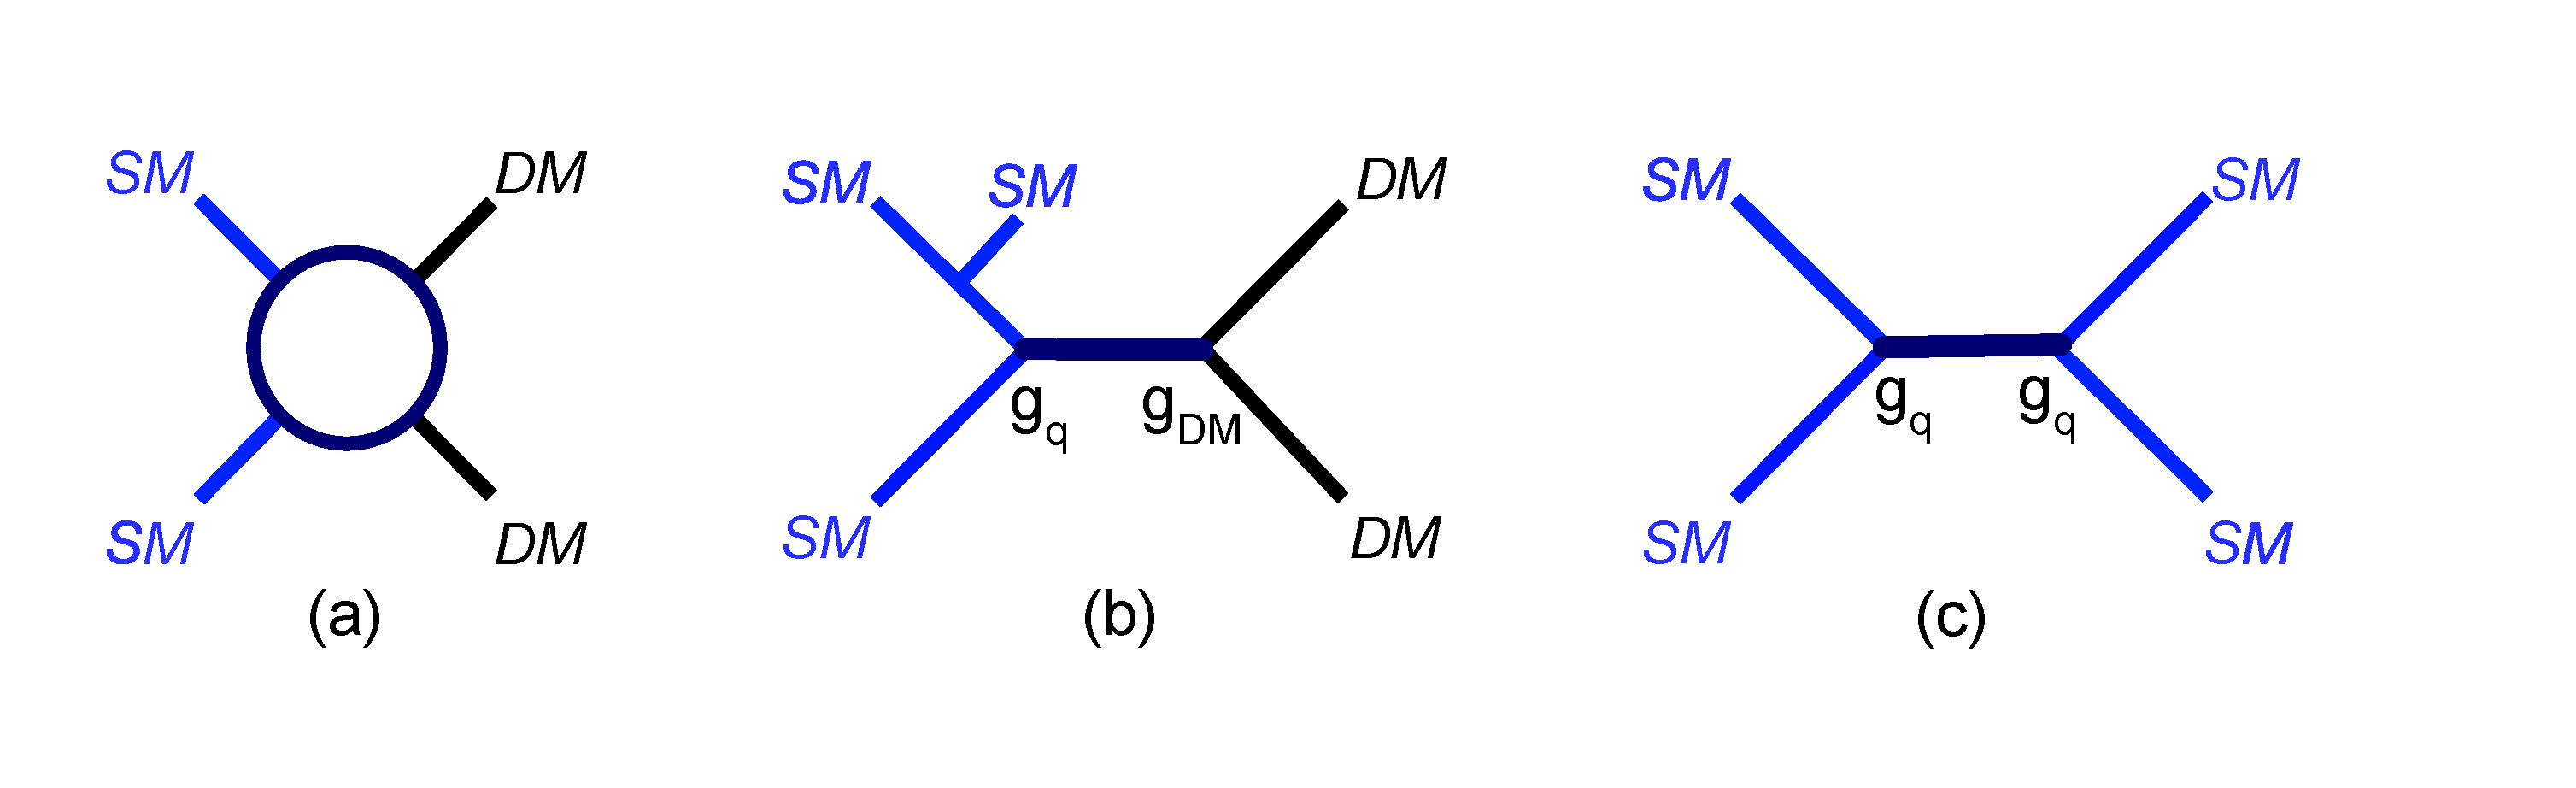
\includegraphics[width=\textwidth]{figures/MonoX.pdf}
\caption{Sketches of (a) the basic Standard Model (SM) - Dark Matter (DM) interaction at colliders in an effective field theory (EFT), (b) its extension as a basic simplified model where a new mediator particle is exchanged in the s-channel (including an additional energetic object radiated from one of the initial state quarks) and (c) the same simplified model where the mediator decays back into SM quarks. The coupling constant characterizing the mediator-quark interaction strenght is denoted as \gq, while the mediator-DM coupling constant is denoted as \gdm. From~\cite{monoXfig}.}
\label{fig:monoX}
\end{figure}

%\subsubsection{Effective Field Theories}

\textbf{Effective field theories} (EFTs)~\cite{Goodman:2010ku, Shoemaker:2011vi} are the simplest possible models of DM production at the LHC beyond those described in Section~\ref{sec:HZPortalModels}. A four-point interaction is used to describe the DM production at the LHC in a low-energy approximation of a full theory, similarly to what done when describing the weak interaction through a Fermi process before the introduction of the W and Z bosons~\cite{Fermi2008}. EFT operators were first widely employed to describe DM reactions at colliders at the Tevatron~\cite{Bai:2010hh,Beltran:2010ww}. They were found advantageous because of their model-independence, and since each of the operators encapsulates the phenomenological characteristics of most known types of SM-DM interaction. A sketch of an EFT process at the LHC is shown in panel (a) of Fig.~\ref{fig:monoX}. 

The only parameter characterizing an EFT operator, in addition to the type of DM particle and to the type of SM-DM interaction, is the scale of the contact interaction $\Lambda$. In the case of a $s-$channel completion of the EFT, this interaction scale is proportional to the mass of the mediator particle. If the scale of the DM interaction is sufficiently low with respect to the mediator mass, the phenomenology is the same for the EFT as for its $s-$channel completion. 
This may not always be the case at the LHC, given the high center-of-mass energy collisions: a better description of both theory and phenomenology can be reached when explicitly including the new particles in the model considered~\cite{Buchmueller:2013dya,DeSimone:2016fbz,Berlin:2014cfa}. Certain EFT operators also may suffer from gauge invariance issues at the electroweak scale~\cite{Bell:2015sza}. 

\begin{marginnote}[]
If a completion of the EFT is not available, procedures describing how to truncate the events where the EFT description is not valid are available~\cite{Racco:2015dxa,Busoni:2014sya,Busoni:2013lha,Busoni:2014haa}. A recommendation on how to present EFT results from LHC searches can be found in~\cite{Abercrombie:2015wmb}.
\end{marginnote}

\textbf{Simplified models of BSM mediation} are a natural step beyond effective operators and still map well to the different types of interactions. 

Simplified models resolve the issue of whether a model-independent EFT description is valid at the LHC, even though they are not complete models themselves (e.g. not all the models used are gauge invariant~\cite{Kahlhoefer:2015bea}). Simplified models can be used for comparisons with non-collider DM searches within a clearly specified theory framework. Their use as benchmark models for Run-2 searches also highlights the strength of the LHC in searching for the visible decays of the mediator particle alongside its decays in DM particles, as detailed in the next chapter. 

For a comprehensive review of WIMP simplified models of DM at the LHC, we refer to~\cite{Arcadi:2017kky}, while~\cite{Abercrombie:2015wmb} presents a prioritized list of simplified models that have been used in early LHC Run-2 searches. The prioritized, compact set of benchmark simplified models in~\cite{Abercrombie:2015wmb}, as well as their parameters, have been discussed and agreed upon during a joint experimental and theory effort called the Dark Matter Forum (DMF), now Dark Matter Working Group within the LHC Physics Centre at CERN (LPCC)~\cite{}. 

\begin{marginnote}[]
The DMF was built starting from the discussion of various communities in Refs.~\cite{Yavin:14092893,Malik:2014ggr,Abdallah:2015ter}. All models covered in~\cite{Abercrombie:2015wmb} are available on the DMF git repository. Add reference. 
\end{marginnote}

In the simplified models chosen as benchmarks for the first LHC Run-2 searches, only one extra particle is added to the the DM and SM particle spectra. In general, this particle mediates the DM-SM interactions. If neutral, the mediator particle is singly-produced at the LHC, and decays in pairs of DM particles due to the $Z_2$ symmetry as well as in pairs of SM particles. If the mediator is colored, it can lead to a $t-$channel exchange between an incoming LHC parton and the DM particle. The phenomenology of colored mediators of DM is akin to that of SUSY models with a squark exchange~\cite{Papucci:2014iwa,An:2013xka,Bell:2012rg} with some differences that we will review later in this section. 

Early LHC searches have initially privileged $s-$channel resonances as benchmark models, as a generalization of the simplest portal models described in the previous section. Resonances decaying in two bodies
%, be those visible or invisible particles, 
are a simple, attractive benchmark to be directly produced at particle collider that has just increased its center-of-mass energy. These resonances can be classified according to their spin: spin-1 vector or axial vector resonances (also called Z'), scalar resonances (termed $\phi$ in the following) and spin-2 vector resonances.

%CD question: introducing parameter scans is too long, so omitted here. 

%General
\textbf{Massive spin-1 bosons with axial or axial vector couplings} to SM and DM particles~\cite{Shoemaker:2011vi} are common in many theories, beyond those of DM mediation. They can be considered as heavy copies of the SM Z boson that arise from breaking of larger gauge groups, and as such they can be contained in larger models. A relevant characteristic of this model for LHC phenomenology is that if the Z' couples to quarks (as it needs to, in order to be produced at the LHC), then it must have visible decays back into quarks. This opens a new avenue for LHC searches of this new particle in dijet signatures, complementing searches for excesses of missing transverse momentum. 
%Parameters
The simplest incarnation of kind of model, where the Z' only couples equally to each kind of quarks and to DM, is fully defined given the nature of the Z' couplings (vector, axial vector or mixed), their magnitude (\gq and \gDM), the mass of the DM particle \mdm and the mediator mass \mmed. The nature of the Z' couplings (vector, axial vector or mixed) does not change the LHC phenomenology, but changes the comparison of LHC results to DD and ID searches. Axial vector are the most widely used LHC benchmarks as DD rates are suppressed. [CD: specify more?]. 
%Problems
In certain region of this parameter space, especially at low mediator masses, the leptophobic Z' model can satisfy the relic density constraints~\cite{Chala:2015ama}. However, if taken in isolation, this model is non-renormalizable, and violates perturbativity in certain regions of the parameter space. 

%General
\textbf{Neutral scalar and pseudoscalar bosons} mediating SM-DM interactions (see e.g. Refs.~\cite{Buckley:2014fba}) take advantage of the theoretical and experimental body of knowledge that led to the recent discovery of another scalar boson, the Higgs boson. Minimal Flavor Violation dictates that the coupling of these new bosons to fermions should be proportional to those of the Higgs boson, and therefore that their visible decays should be dominated by heavy-flavor quarks. Other parallels with LHC Higgs phenomenology are the importance of loop-induced couplings to gluons in the production of scalar and pseudoscalar mediators for the lowest-order diagrams of this process~\cite{Haisch:2015ioa} and the associated production of the mediator together with heavy flavour quarks~\cite{Buckley:2014fba}.  
%Parameters
The model is fully defined given the mass of the DM particle and of the mediator, the nature of the $\phi$-DM couplings (\gdm) and $\phi$-fermion (\gq) couplings. Following the convention in~\cite{Abercrombie:2015wmb}, \gq is a pre-factor to the Yukawa couplings of the mediator to fermions and it is considered equal for all quarks in early LHC searches. 
The LHC kinematics of models with scalar and pseudoscalar mediators assuming the same couplings is degenerate. Since the pseudoscalar model has been favoured for the interpretation of the DAMA and galactic center excess~\cite{Arina:2014yna,Agrawal:2014una}, LHC searches have privileged this choice. 
%Problems
If the mediators are pure SM singlets, the model is not invariant under $SU(2)_L$. To restore gauge invariance, the mediator needs to mix with the Higgs sector, introducing further complexity of interactions. However, as we will see in Sec.~\ref{sec:LessSimplifiedModels}, this complexity does not translate into significant changes in the LHC phenomenology of these models. 

%They are the favoured explanation for the galactic center excess
%

\textbf{Colored scalar and pseudoscalar bosons} mediating SM-DM interactions

\subsubsection{Less simplified models}
\label{sec:LessSimplifiedModels}


\subsection{Supersymmetric models}
\label{sec:SUSYModels}

\subsection{Long-lived particle models}
\label{sec:LLPModels}